\documentclass[10pt]{article}
\def\d{{\fontencoding{T1}\selection\dj}}
\def\D{{\fontencoding{T1}\selection\DJ}}
\usepackage{hyperref}
\usepackage{graphicx}
\title{Analiza skupa podataka Network Intrusion Data\\~\\ \small{ Seminarski rad u okviru kursa\\Istra\v zivanje podataka 1} \\ \small{Matemati\v cki fakultet}}
\author{Marina Pilipovi\' c 115/2015\\Vladana  Djordjevi\' c 89/2015}
\date{Septembar 2018.}
\begin{document}
\maketitle

\section{Uvod u podatke}
Skup podataka koji \' cemo obradjivati kori\v s\' cen je na KDD (Knowledge Discovery and Data Mining) kupu odr\v zanom 1999. godine. Podaci se odnose na napadanje mre\v za i mogu se na\' ci \href{http://kdd.ics.uci.edu/databases/kddcup99/kddcup99.html}{ovde}. Medju navedenim linkovima mi smo koristile 10\% ukupnog skupa (kddcup.data\_10\_percent), radi br\v zeg izvr\v savanja algoritama.

\section{Analiza i pretprocesiranje}
Podaci se nalaze u jednoj tabeli koja se sastoji od 494021 instanci, gde svaka instanca predstavlja jedan zapis o konekciji. Svaka konekcija je opisana pomo\' cu 41 atributa i ozna\v cena kao napad na mre\v zu odredjenog tipa ili kao normalan saobra\' caj.
Svi atributi se mogu podeliti u tri grupe, mi smo za svaku grupu izdvojile najva\v znije atribute i prikazale ih tabelarno:


\begin{enumerate}
\item osnovni atributi: u ovoj kategoriji se nalaze svi atributi koji mogu biti izdvojeni iz TCP/IP konekcije.

\begin{tabular}{ |c|c|c| } 
 \hline
 ime atributa & opis & tip\\
 \hline
 protocol\_type & tip protokola & diskretan\\
 \hline
 service & internet servis na destinaciji & diskretan\\
 \hline
 src\_bytes & broj bajtova podataka od izvora do destinacije & neprekidan\\
 \hline
 flag & status konekcije(normalan ili gre\v ska) & diskretan\\
 \hline
\end{tabular}
\item atributi saobra\'caja: ova kategorija uklju\v cuje atribute koji su izra\v cunati uzimaju\' ci u obzir vremenski inteval i podeljena je u dve grupe ("same host" i  "same service").

\footnotesize{
\begin{tabular}{ |c|c|c| }
\hline
ime atributa & opis & tip\\
\hline
count & broj konekcija ka istom hostu kao i trenutna konekcija u poslednje 2 sekunde & neprekidan\\
\hline
serror\_rate & procenat konekcija koji imaju SYN gre\v ske & neprekidan\\
\hline
rerror\_rate & procenat konekcija koje imaju REJ gre\v ske & neprekidan\\
\hline
same\_srv\_rate & procenat konekcije ka istom servisu & neprekidan\\
\hline
diff\_srv\_rate & procenat konekcije ka razli\v citim servisima & neprekidan\\
\hline
\end{tabular}
}

\normalsize{
\item atributi sadr\v zaja: uklju\v cuje atribute koji pretra\v zuju sumnjiva pona\v sanja u podacima.}

\begin{tabular}{ |c|c|c| }
\hline
ime atributa & opis & tip\\
\hline
num\_failed\_logins & broj neuspelih poku\v saja prijavljivanja & neprekidan\\
\hline
logged\_in & 1 - za uspe\v sno prijavljivanje, 0 - ina\v ce & diskretan\\
\hline
su\_attempted & 1 - ako je poku\v sana komanda "su root", 0 - ina\v ce & diskretan\\
\hline
num\_file\_creations & broj operacija kreiranja fajlova & neprekidan\\
\hline

\end{tabular}

\end{enumerate}

Analizu skupa podataka zapo\v cinjemo \v cvorom CSV Reader (slika 2.1), kojim u\v citavamo podatke. Da bismo se pozabavili nedostaju\' cim vrednostima moramo prvo da proverimo da li ih ima. U tu svrhu koristimo \v cvor Missing Value kome sve tri vrednosti polja za obradu nedostajucih vrednosti postavljamo na "Remove Row*". Time obezbedjujemo da \'ce nedostaju\' ce vrednosti, ako se u bilo kom redu jave (bilo kategori\v ckih, bilo numeri\v ckih atributa), biti uklonjene. Nakon pokretanja \v cvora uporedjujemo broj redova izlazne i originalne tabele. S obzirom na to da se broj redova nije promenio dolazimo do zaklju\v cka da podaci ne sadr\v ze nedostaju\' ce vrednosti.
S obzirom na to da obrada skoro 500000 instanci zahteva mnogo vremena, koristimo \v cvor Partitioning da bismo izdvojili 10\% celokupnog skupa, \v cime smanjujemo vreme izvr\v savanja. Kao parametar smo zadali stratifikovano uzorkovanje na osnovu ciljne klase (class).

\begin{center}
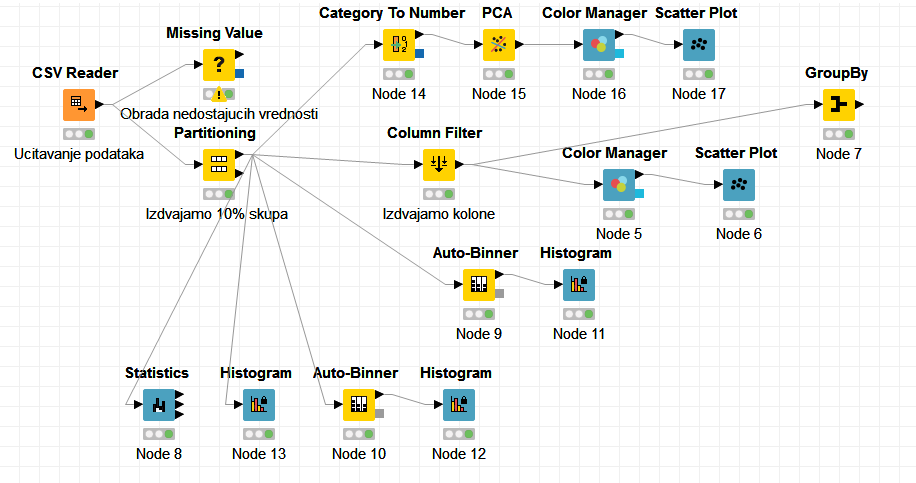
\includegraphics[width = \textwidth]{slika1}
slika 2.1: analiza i pretprocesiranje skupa podataka\\
\end{center}

Da bismo se upoznali sa numeri\v ckim karakteristikama podataka koristimo \v cvor Statistics. Na slikama 2.2, 2.3, 2.4 i 2.5 mogu se videti neke od va\v znijih karakteristika.

\begin{center}
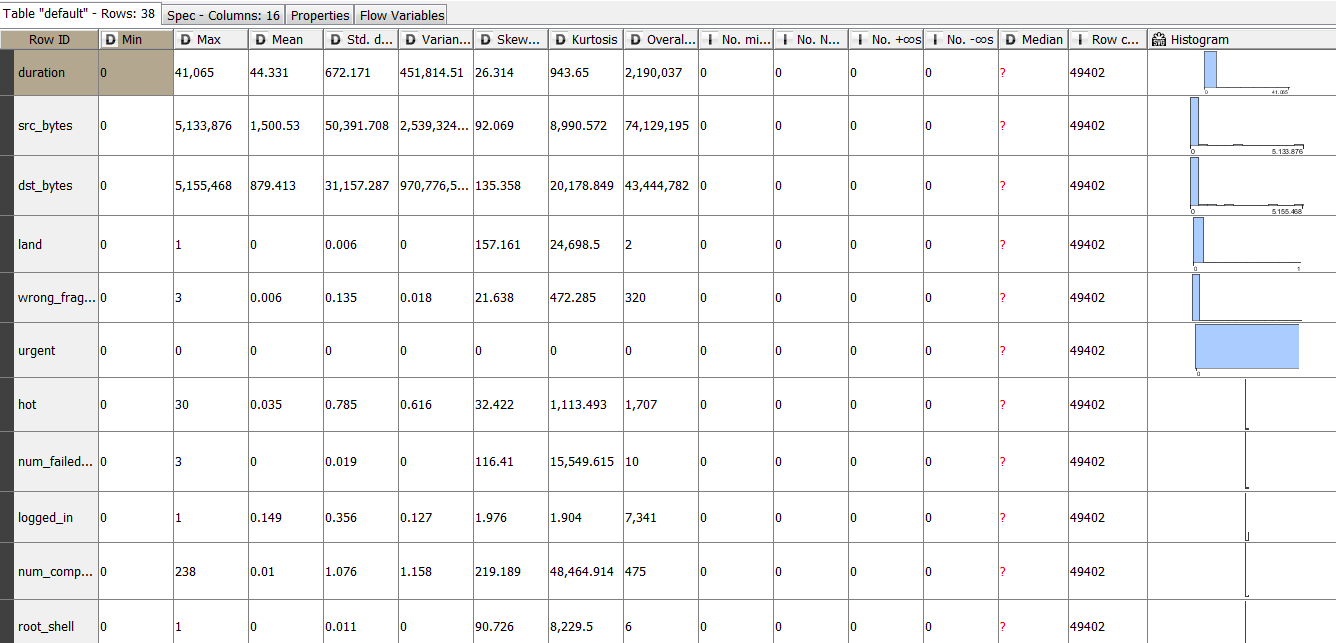
\includegraphics[width = \textwidth, height = 7.5cm]{slika2}
slika 2.2: statistike atributa\\
\end{center}

\begin{center}
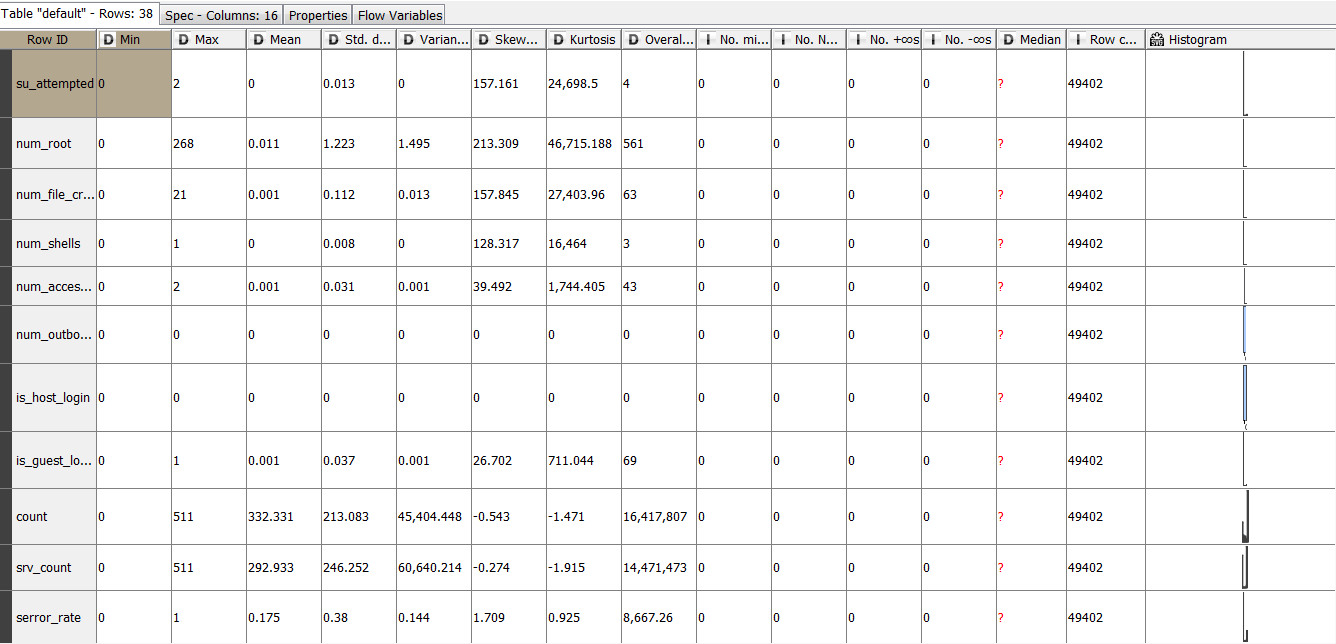
\includegraphics[width = \textwidth,  height = 7.5cm]{slika3}
slika 2.3: statistike atributa\\
\end{center}

\begin{center}
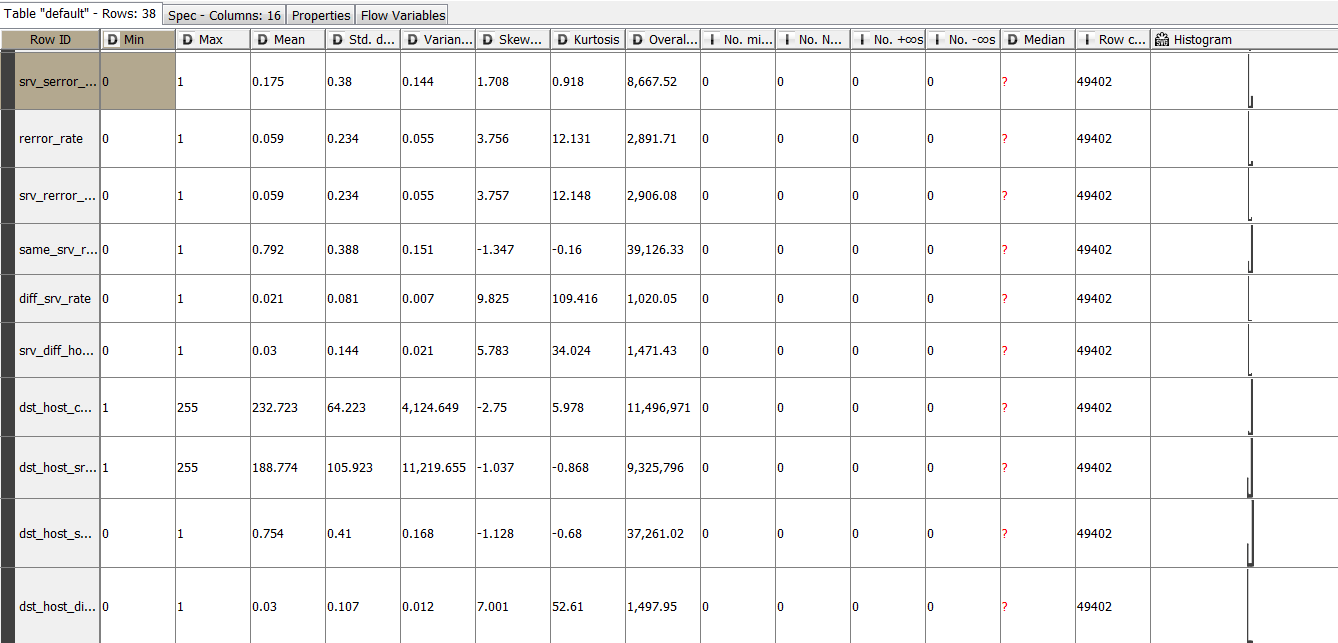
\includegraphics[width = \textwidth,  height = 7.5cm]{slika4}
slika 2.4: statistike atributa\\
\end{center}

\begin{center}
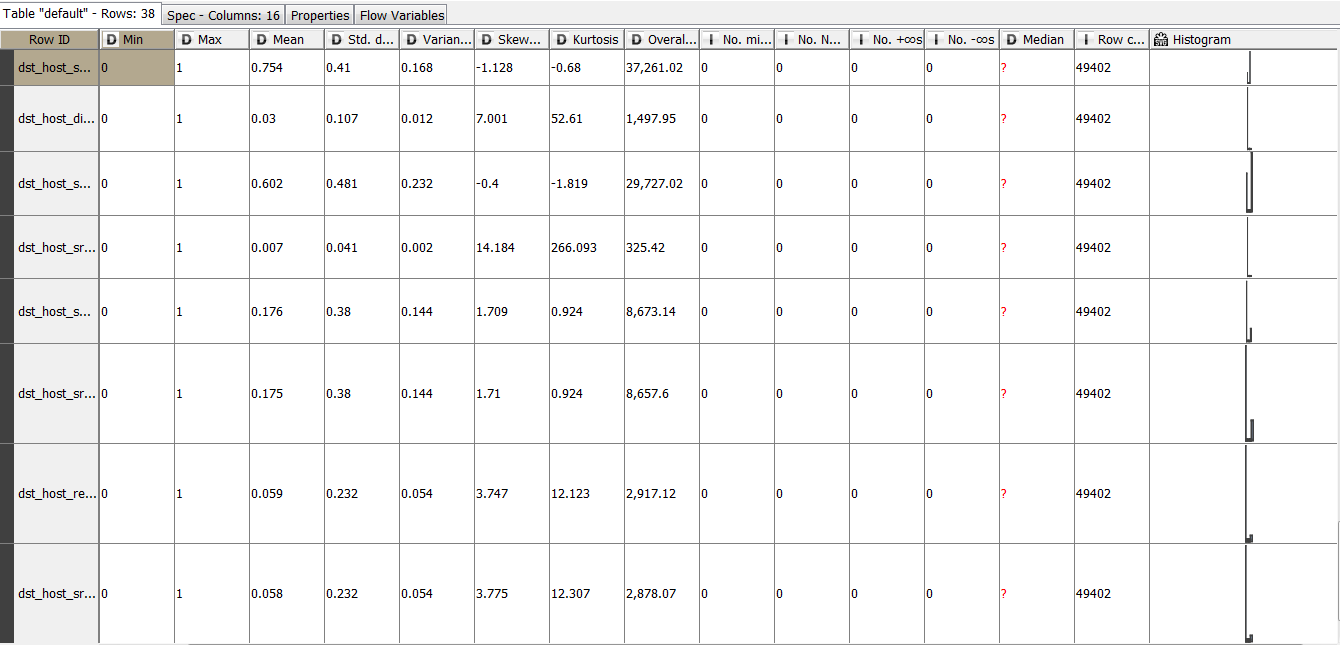
\includegraphics[width = \textwidth,  height = 7cm]{slika5}
slika 2.5: statistike atributa\\
\end{center}

Na osnovu histograma mo\v zemo da zaklju\v cimo da se u ve\' cini atributa veliki broj puta pojavljuje jedna do nekoliko razli\v citih vrednosti. Zna\v ci da su atributi takvi da se u njima ne javlja mno\v stvo razli\v citih vrednosti. To zaklju\v cujemo na osnovu toga \v sto se u histogramima ne javljaju vrednosti rasporedjene du\v z njegove x-ose, ve\' c su vrednosti uglavnom skoncentrisane na jednom mestu. Nekoliko atributa predstavlja flegove, \v cije vrednosti mogu biti jedino 0 i 1. Neki izra\v zavaju procente u opsegu [0,1].

\subsection{Obrada outlier-a}

Za obradu outlier-a na\v sih podataka KNIME nije bio pogodan izbor, s obzirom na to da je vizuelizacija outlier-a pomo\' cu Box Plot \v cvora bila te\v sko \v citljiva. Stoga smo koristile programski jezik Python i biblioteku za ma\v sinsko u\v cenje numpy da bismo izdvojile vrednosti van granica. 

\section{Vizualizacija}

Za vizualizaciju podataka koristimo \v cvor Histogram. \v Zelimo da vidimo koliko se u proseku \v salje i prima bajtova u odnosu na razli\v cite protokole. Zato smo kao kolonu koju \' cemo "razlo\v ziti" na razli\v cite vrednosti stavili atribut "protocol\_type" (tip protokola), a kolone po kojima \' cemo vr\v siti agregaciju smo stavili da budu src\_bytes (broj bajtova od izvora do odredi\v sta) i dst\_bytes (broj bajtova od odredi\v sta do izvora).

\begin{center}
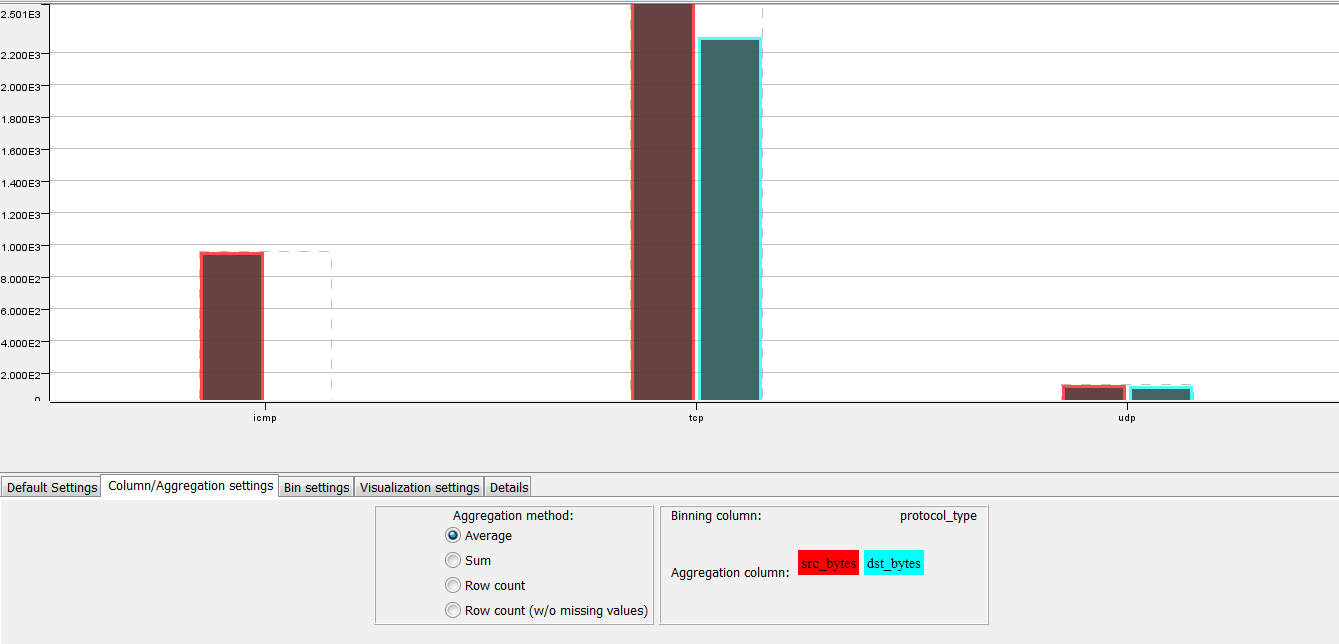
\includegraphics[width = \textwidth,  height = 7.5cm]{vizuelizacija1}
slika 3.1: Prose\v can broj poslatih i primljenih bajtova po protokolu\\
\end{center}

Uo\v cavamo da se mnogo ve\' ci broj bajtova po proseku prenosi preko tcp protokola (i icmp u odredjenoj meri) nego preko udp. Takodje, kod konekcija koje su koristile icmp protokol nije bilo primljenih bajtova (od odredi\v sta do izvora). Sve to mo\v ze da nam bude zanimljivo, s obzirom na to da se neki napadi sastoje isklju\v civo od ogromnog broja poslatih bajtova. Na ovaj na\v cin mo\v zemo dovesti u vezu protokole konekcije sa napadima na mre\v ze.\\
Potom smo podelile sve mogu\' ce vrednosti atributa dst\_bytes u 5 "korpi" po frekvenciji koris\' ci \v cvor Auto-Binner i te vrednosti prosledili Histogram-u jer smo \v zelele da vidimo u kom opsegu se nalazi broj bajtova koji se najvi\v se prenosi po konekciji.

\begin{center}
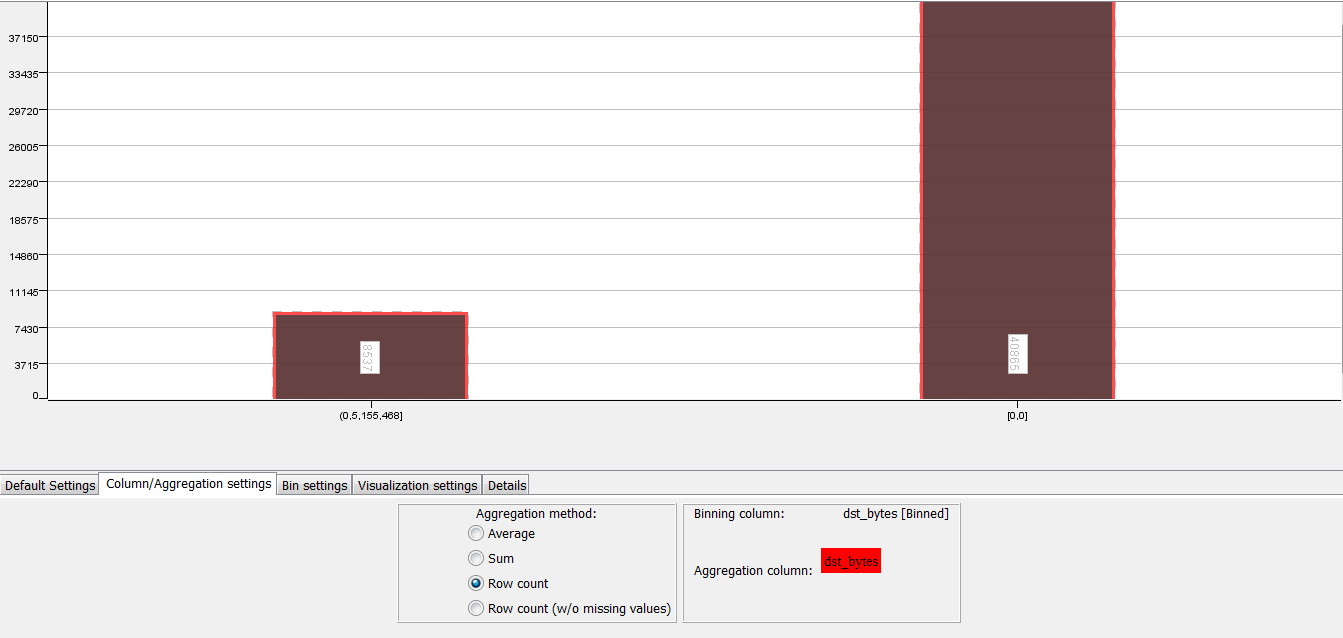
\includegraphics[width = \textwidth,  height = 7.5cm]{vizuelizacija2_dst}
slika 3.2: Broj instanci po razli\v citom opsegu vrednosti atributa dst\_bytes\\
\end{center}

Kao rezultat smo dobile dve "korpe", jer ovaj atribut ne sadr\v zi veliki broj razli\v citih vrednosti da bi se mogle na toliko "korpi" razlo\v ziti. Takodje, vidimo da se u najve\' cem broju konekcija (instanci) \v salje 0 bajtova od odredi\v sta do izvora.
Isti postupak smo primenile na atribut src\_bytes.

\begin{center}
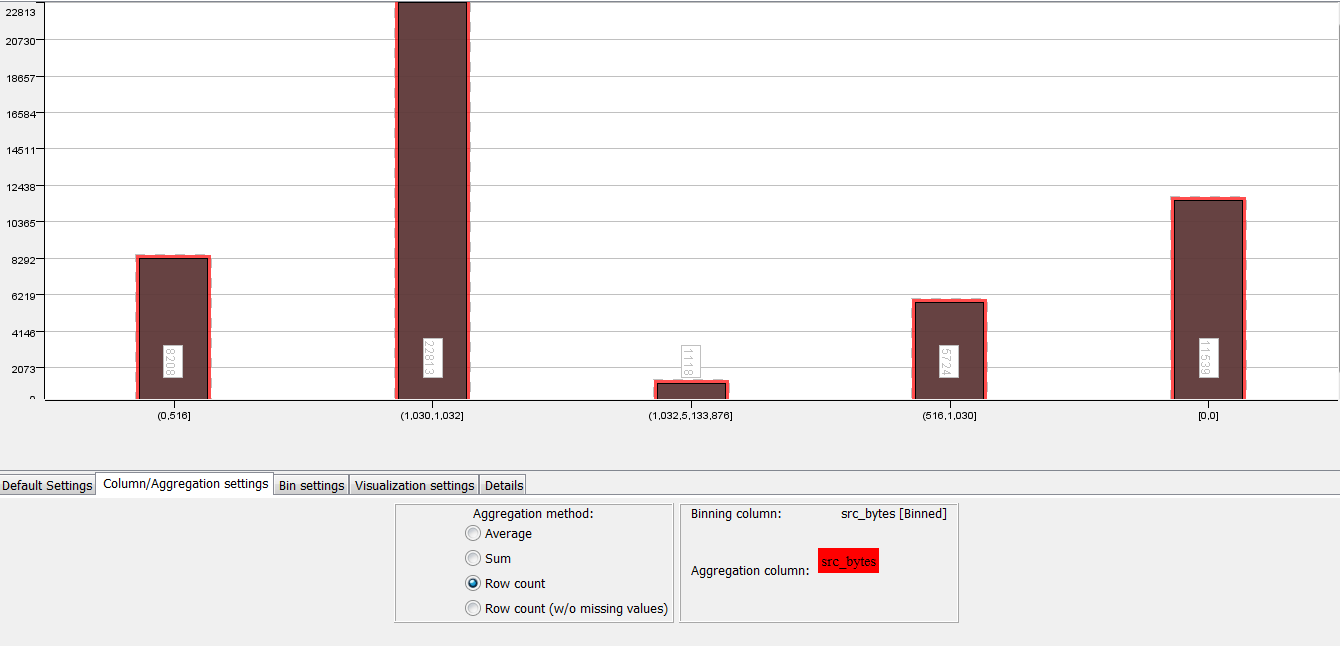
\includegraphics[width = \textwidth,  height = 7cm]{vizuelizacija3_src}
slika 3.3: Broj instanci po razli\v citom opsegu vrednosti atributa dst\_bytes\\
\end{center}

Ovde ve\' c jesmo dobile 5 korpi usled \v cinjenice da ovaj atribut sadr\v zi ve\' ci broj razli\v citih vrednosti.\\
Nakon toga, zanimao nas je odnos tipa protokola (protocol\_type) u odnosu na procenat "SYN" (serror\_rate) i "REJ" (rerror\_rate) gre\v ske. Prvo smo pomo\' cu \v cvora Column Filter izdvojili pomenute atribute, nakon toga smo u \v cvoru Color Manager dodelili boje razli\v citim tipovima protokola, a onda smo rezultate iscrtale pomo\' cu \v cvora Scatter Plot (JFreeChart).

\begin{center}
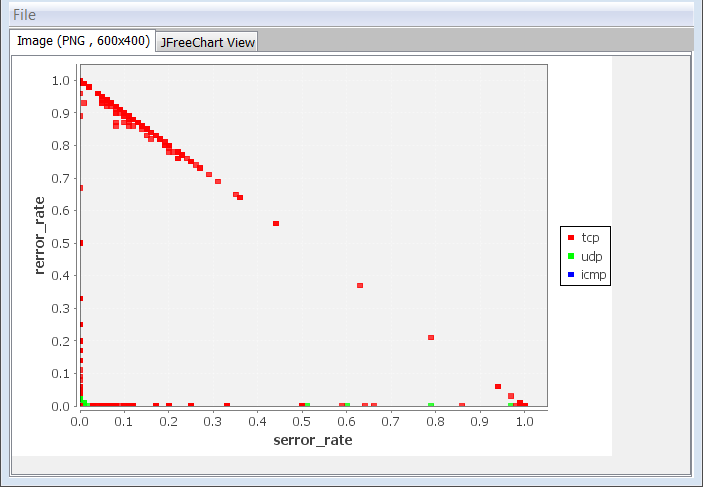
\includegraphics[width = \textwidth,  height = 9cm]{vizuelizacija4_nova}
slika 3.4: Razli\v citi protokoli u odnosu na procenat "SYN" i "REJ" gre\v ske\\
\end{center}

Prime\' cujemo da se ve\' cina gre\v saka javila u okviru tcp protokola, a nijedna u okviru icmp protokola. Da bismo to proverile iskoristile smo \v cvor GroupBy koji grupi\v se redove tabele po jedinstvenim vrednostima u izabranim atributima, a mi smo izabrale upravo tri pomenuta atributa.

\begin{center}
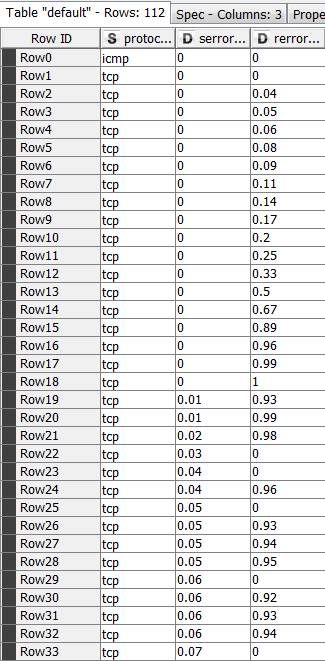
\includegraphics[height = 9cm]{v5_1}
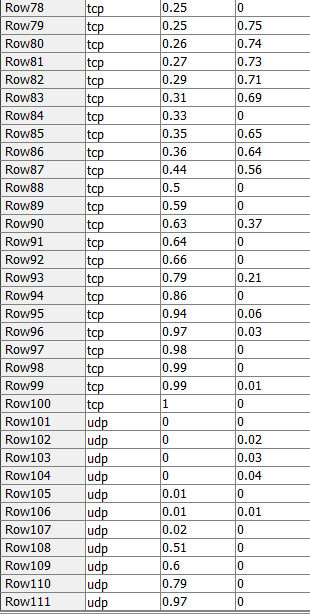
\includegraphics[height = 9cm]{v5_2}\\
slika 3.5: Deo tabele koji predstavlja grupisane instance po jedinstvenim vrednostima atributa\\
\end{center}

Kao \v sto mo\v zemo da vidimo na osnovu tabele icmp zaista ima 0 procenata i "SYN" i "REJ" gre\v ske kao i da se u udp konekciji javlja mali procenat istih. Dakle, ove vrste gre\v saka se najvi\v se javljaju u okviru konekcije sa tcp protokolom, a one su karakteristi\v cne za DoS napade. Ono \v sto je vrlo interesantno je to da se napadi na mre\v ze mogu vi\v se dovesti u vezu sa tcp protokolom, koji omogu\' cava sigurniju vezu, nego sa udp protokolom koji nije toliko siguran.\\ 
Hteli smo i da proverimo na koji na\v cin smanjivanje dimenzionalnosti na\v sim podacima uti\v ce na krajnji ishod. U tu svrhu smo iskoristile \v cvor PCA, kome smo kao parametar stavile da \v zelimo 95\% informacija da sa\v cuva, medjutim, pre njegove primene, \v cvorom Category To Number smo tri kategori\v cka atributa - protocol\_type, service i flag - prebacile u numeri\v cke jer PCA algoritam radi samo sa numeri\v ckim vrednostima. Na taj na\v cin smo omogu\' cile da PCA koristi sve atribute u procesu smanjivanja dimenzionalnosti. Nakon toga smo povezale \v cvor Color Manager koji je dodelio boju svim mogu\' cim vrednostima ciljne klase i potom smo rezultat prikazali pomo\' cu \v cvora Scatter Plot (JFreeChart).

\begin{center}
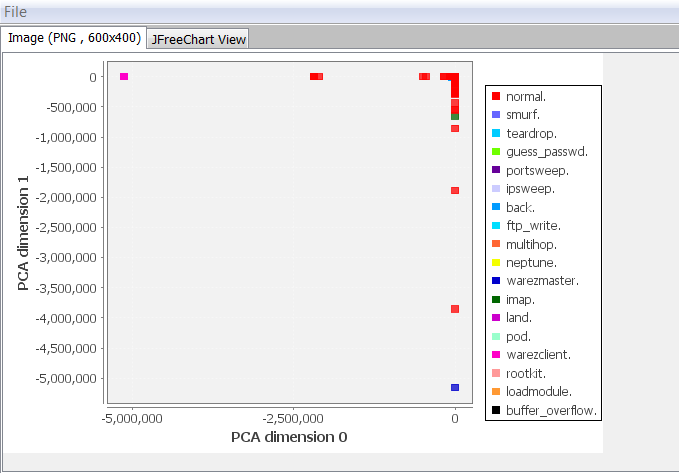
\includegraphics[width = \textwidth,  height = 7.5cm]{vizuelizacija6}
slika 3.6: Razli\v citi protokoli u odnosu na procenat "SYN" i "REJ" gre\v ske\\
\end{center}

Mo\v zemo da zaklju\v cimo da se u najve\' cem broju slu\v cajeva javlja normalna konekcija.

\section{Pravila pridru\v zivanja}

Da bismo primenili pravila pridru\v zivanja na na\v se podatke potrebno je prvo da ih u\v citamo, za \v sta koristimo CSV Reader, a potom da napravimo kolekcijsku kolonu koja sadr\v zi elemente koji su nam od zna\v caja za pravila pridru\v zivanja. Kolekcijsku kolonu pravimo koriste\' ci \v cvor Create Collection Column kome zadajemo da uklju\v ci atribute: protocol\_type, service, flag (status konekcije), count (broj konekcija ka istom hostu kao i trenutna konekcija u poslednje dve sekunde) i serror\_rate (procenat konekcija koje imaju "SYN" gre\v sku). Ovo su atributi koji su zna\v cajni za DoS napad, pa nas zanima njihov medjusobni odnos zarad boljeg razumevanja samih napada. 

\begin{center}
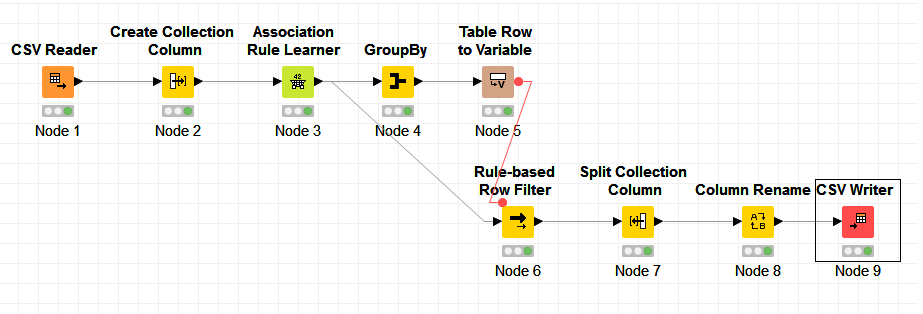
\includegraphics[width = \textwidth]{PP1}
slika 4.1: pravila pridru\v zivanja\\
\end{center}

Nakon toga smo pokrenuli \v cvor Association Rule Learner kome smo parametre podesili na slede\' ci na\v cin:

\begin{center}
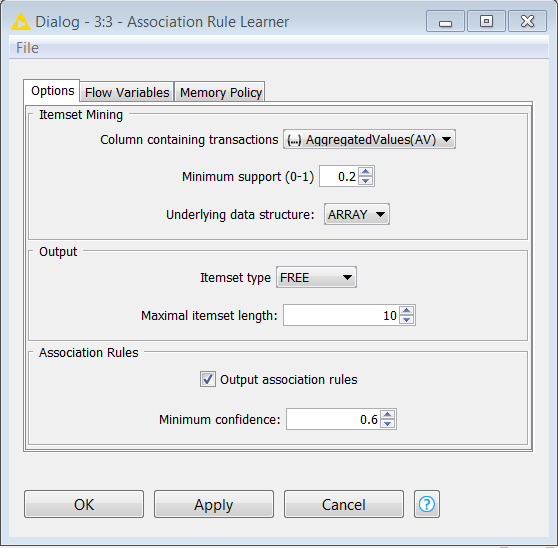
\includegraphics[scale = 0.75]{PP2}\\
slika 4.2: pode\v savanje parametara \v cvora Association Rule Learner\\
\end{center}

Kao rezultat smo dobili slede\' ca pravila pridru\v zivanja:

\begin{center}
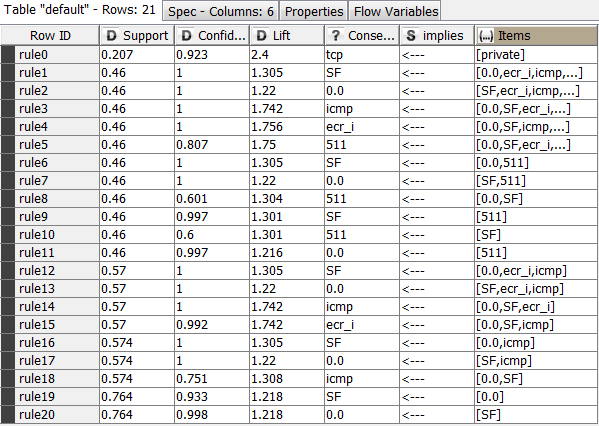
\includegraphics[scale = 0.8]{PP3novo}\\
slika 4.3: izlaz iz \v cvora Association Rule Learner\\
\end{center}

U ovim pravilima nailazimo na neke podatke koje smo ve\' c videli, npr. ukoliko se koristi icmp protokol procenat greske u konekciji \' ce biti 0. Takodje, nailazi se na neke o\v cekivane rezultate - ako je konekcija zavr\v sena sa uspehom (flag = SF), procenat gre\v ske \' je 0 i obrnuto.
Zanimljivo je u pravilima koju su vezana za uspe\v sne konekcije javlja 511 kao broj konekcija ka istom hostu kao i trenutna konekcija u poslednje dve sekunde. Taj broj uslovljava uspe\v sne konekcije, kao \v sto i uspe\v sne konekcije uslovljavaju njega. Sli\v cno kao i broj 511, tako se i ecr\_i servis javlja u okviru uspe\v sno izvr\v senih konekcija. Iz dobijenih pravila se, medjutim, ne mo\v ze izvu\' ci \v sta uslovljava napade, ve\' c su samo dobijene informacije o normalnom saobra\' caju.\\
Zanima nas koja su pravila najbolja po podr\v sci i lift meri, tj. koja pravila imaju najve\' cu vrednost tih "statistika". Da bismo ih izdvojili prvo pronalazimo maksimalnu vrednost podr\v ske i lift mere, uz pomo\' c \v cvora GroupBy. U pode\v savanjima postavljamo da ne uklju\v cujemo nijedan atribut i da izdvajamo Maximum za Support i Lift. Kao izlaz iz tog \v cvora dobijamo:

\begin{center}
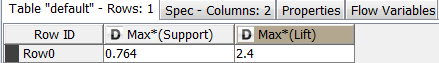
\includegraphics[width = \textwidth]{PP4}
slika 1: analiza i pretprocesiranje skupa podataka\\
\end{center}

Nakon toga koristimo \v cvor Table Row to Variable koji \' ce nam dobijene vrednosti pretvoriti u promenljive kojima mo\v zemo da baratamo u \v cvoru Rule-based Row Filter. U njemu zadajemo da nam se u rezultat uklju\v ce samo oni redovi koji sadr\v ze date maksimalne vrednosti podr\v ske i lift mere. Dobijamo:

\begin{center}
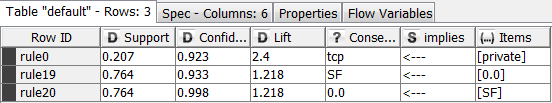
\includegraphics[width = \textwidth]{PP5}
slika 1: analiza i pretprocesiranje skupa podataka\\
\end{center}

Ako dobijene rezultate \v zelimo da ispi\v semo u csv fajl moramo prvo da transformi\v semo podatke u tabeli. Prvo je potrebno kolekcijsku kolonu razbiti na razli\v cite kolone. Bez obzira na to sto na\v sa kolekcija u svakom polju sadr\v zi samo jedan element, CSV Writer ne zna to da isp\v se na izlaz dokle god je kolekcijskog tipa, dakle razbijamo je \v cvorom Split Collection Column. Prime\' cujemo da je tip kolone Consequent nepoznat, \v sto je logi\v cno s obzirom na to da se u njoj nalaze vrednosti razli\v citih tipova. Potrebno je postaviti tip kolone da bi se tabela mogla ispisati na izlaz, za to koristimo \v cvor Column Rename koji sadr\v zi opciju za promenu tipa kolone. Nakon \v sto smo tip Consequent kolone postavili na String mo\v zemo uz pomo\' c \v cvora CSV Writer da ispi\v semo rezultate na izlaz.

\section{Klasterovanje}

Pre primene algoritama za klasterovanje smo smanjile broj instanci zarad br\v zeg izvr\v savanja algoritama. To smo postigle uz pomo\' c \v cvora Partitioning kome smo kao parametre zadale da \v zelimo 0.2\% skupa i stratifikovano uzorkovanje. S obzirom na to da koristimo algoritme koji koriste Euklidsko rastojanje bilo je potrebno prethodno normalizovati podatke, \v cvorom Normalizer, da ne bi neki atributi vi\v se uticali na proces klasterovanja. 

\begin{center}
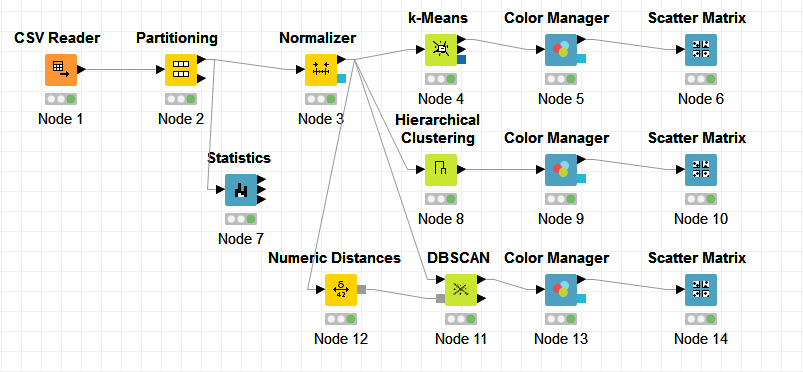
\includegraphics[width = \textwidth]{Klaster1}
slika 5.1: klasterovanje\\
\end{center}

Prvo smo primenile \v cvor k-Means koji primenjuje algoritam k-sredina. Kao atribute po kojima \v zelimo da vr\v simo klasterovanje smo izabrale count, srv\_count, dst\_host\_count jer su jedine vrednosti koji nisu ili 0 ili 1, ili u opsegu [0,1]. Smatrale smo da \' ce nam to lep\v se vizuelno prikazati klastere, jer ti atributi sadr\v ze razli\v citije vrednosti. Parametre smo postavile na slede\' ci na\v cin:

\begin{center}
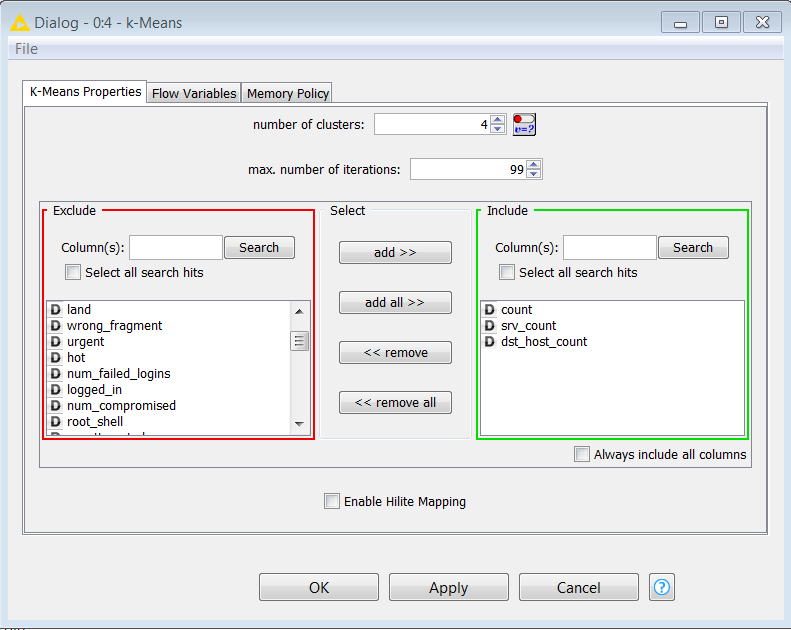
\includegraphics[width = \textwidth, height = 6.5 cm]{Klaster3}
slika 5.2: pode\v savanje parametara \v cvora k-Means\\
\end{center}

\begin{center}
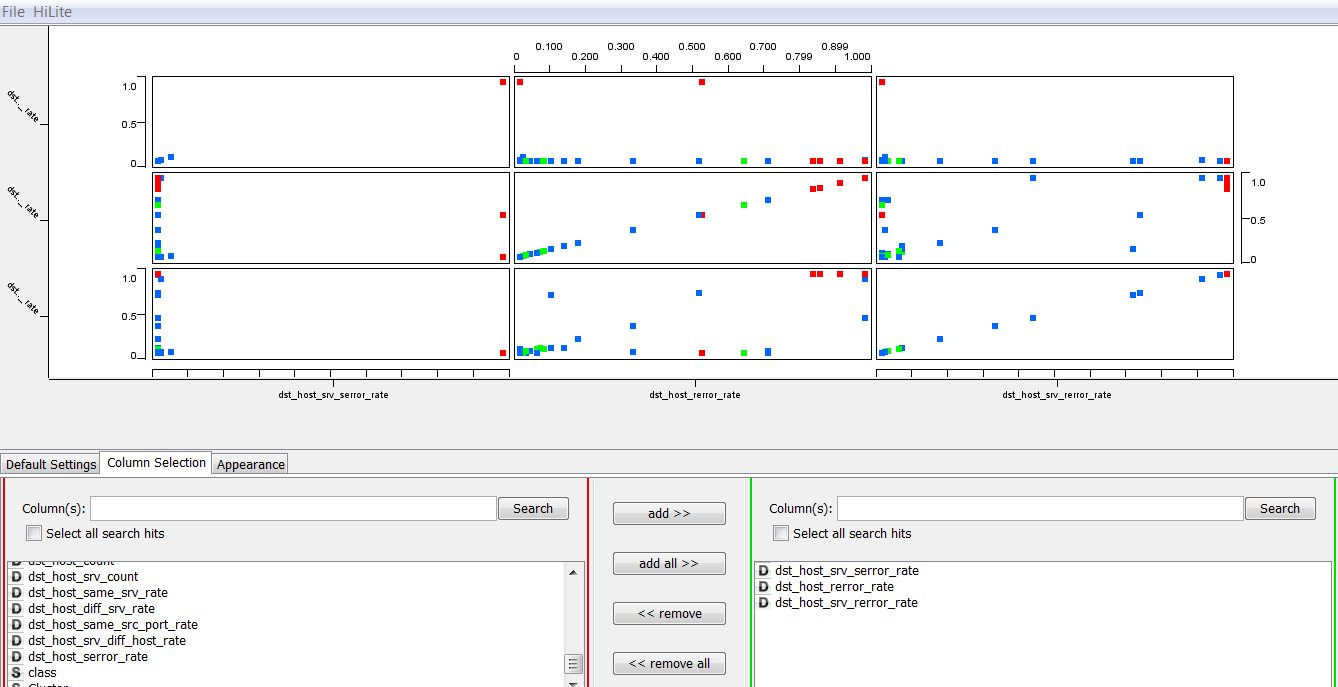
\includegraphics[width = \textwidth]{Klaster4}
slika 5.3: primer lo\v sijeg modela klasterovanja\\
\end{center}

Nakon primene ovog algoritma \v cvorom Scatter Matrix smo prikazale atribute dst\_host\_srv\_serror\_rate, dst\_host\_serror\_rate, dst\_host\_srv\_rerror\_rate. U ovom slu\v caju smo dobile relativno lo\v s model. Klasteri su razbacani i ne mogu se izdvojiti neke korisne informacije.

\begin{center}
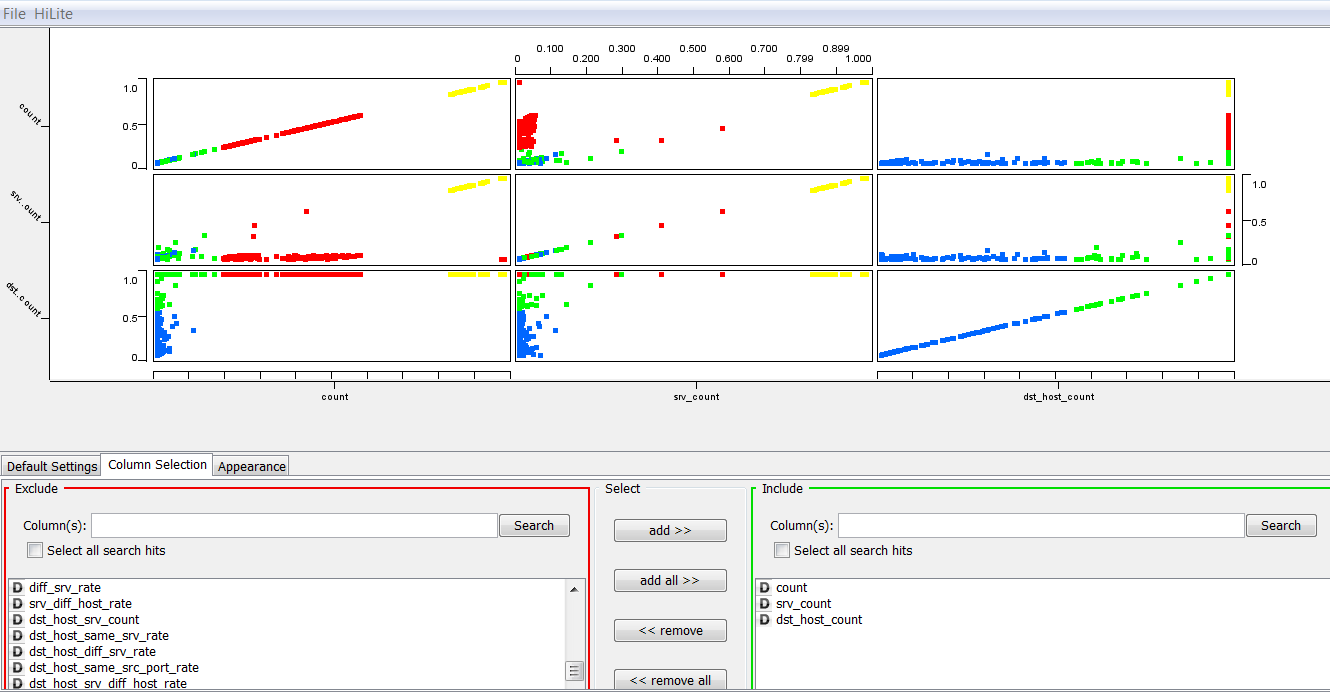
\includegraphics[width = \textwidth]{Klaster2}
slika 5.4: primer boljeg modela klasterovanja\\
\end{center}

Kada smo kao atribute koje \v zelimo da prika\v zemo izabrale upravo atribute koje smo koristile za pravljenje klastera - count, srv\_count, dst\_host\_count - dobile smo bolji model. Na slici se mogu uo\v citi razdvojene celine koje predstavljaju klastere. Najbolja podela se vidi u donjem levom uglu matrice po atributima count i dst\_host\_count. Podaci se prostiru du\v z y-ose i du\v z prave $x = 1$, jer ve\' cina podataka ima vrednosti 0 ili 1, ili eventualno neku vrednost izmedju.\\
Nakon toga smo primenili hijerarhijsko klasterovanje uz pomo\' c \v cvora Hierarchical Clustering. Ponovo smo izabrale iste atribute, zbog gore navedenog razloga. Takodje, kao rastojanje smo izabrale Manhattan, prvenstveno da bismo videle razliku u odnosu na Euklidsko koje je kori\v s\' ceno u k-sredina, a i zato \v sto nam se \v cini da obliku na\v sih podataka vi\v se odgovara to rastojanje.

\begin{center}
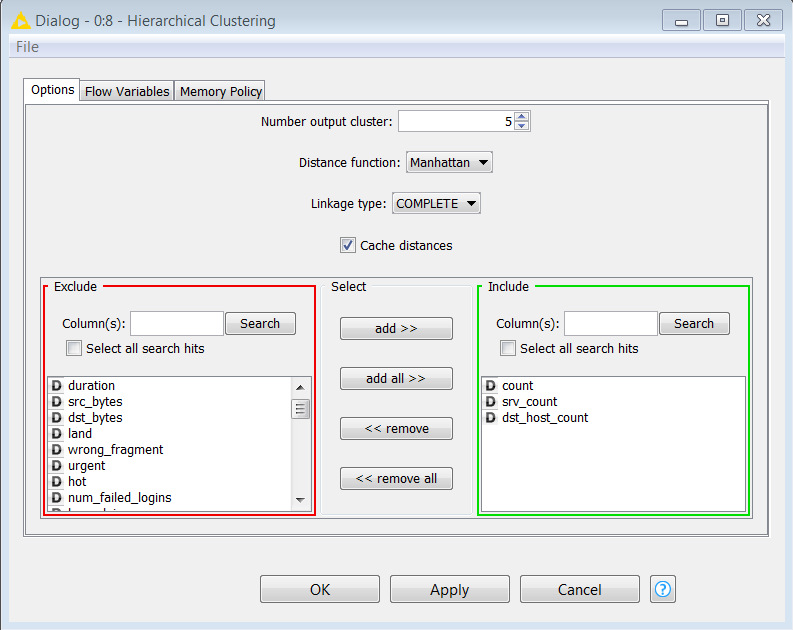
\includegraphics[width = \textwidth, height = 8 cm ]{Klaster5}
slika 5.5: pode\v savanje parametara \v cvora Hierarchical Clistering\\
\end{center}

\begin{center}
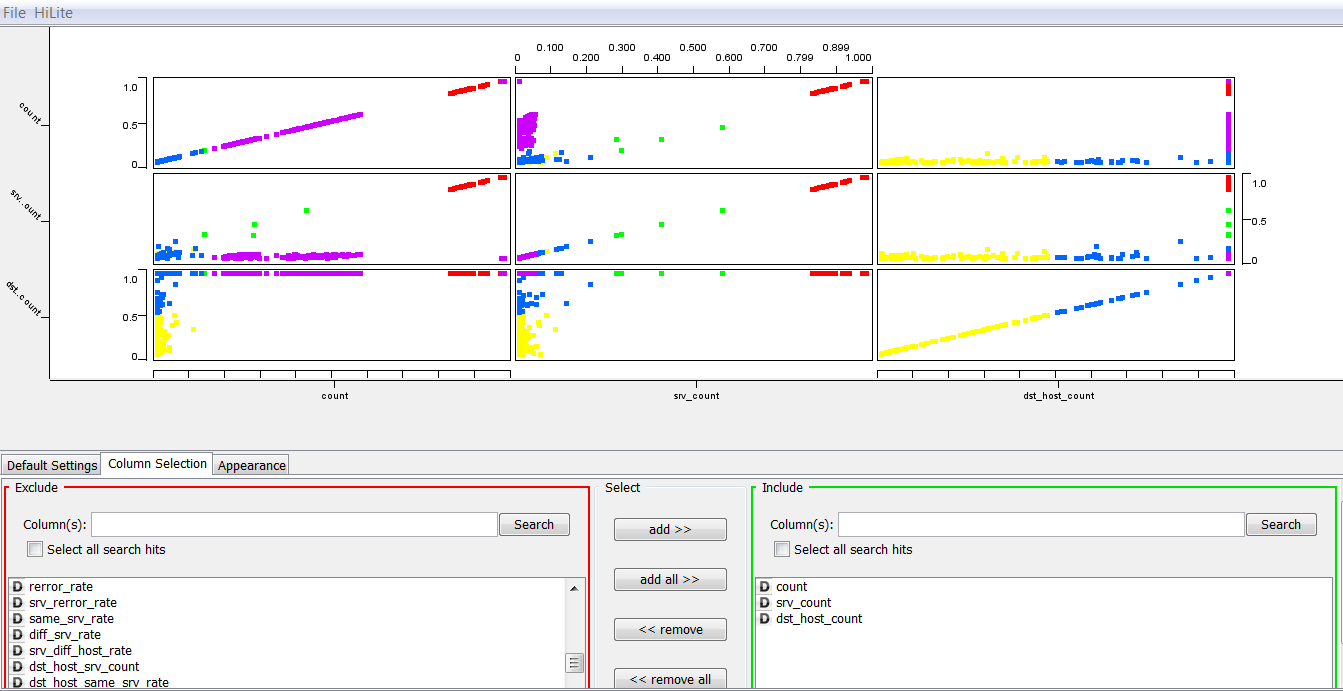
\includegraphics[width = \textwidth,height = 6 cm]{Klaster6}
slika 5.6: primer modela dobijenog hijerarhijskim klasterovanjem\\
\end{center}

Dobili smo isti rezultat kao i primenom algoritma k-sredina.\\
Da bismo primenile algoritam DBSCAN potrebno je prvo zadati model \v cvorom Numeric Distances. Biramo iste atribute kao i u prethodna dva puta, a kao meru rastojanja smo izabrale Maximum. U \v cvoru DBSCAN epsilon postavimo na 0.1, a minimalan broj ta\v caka na 6.

\begin{center}
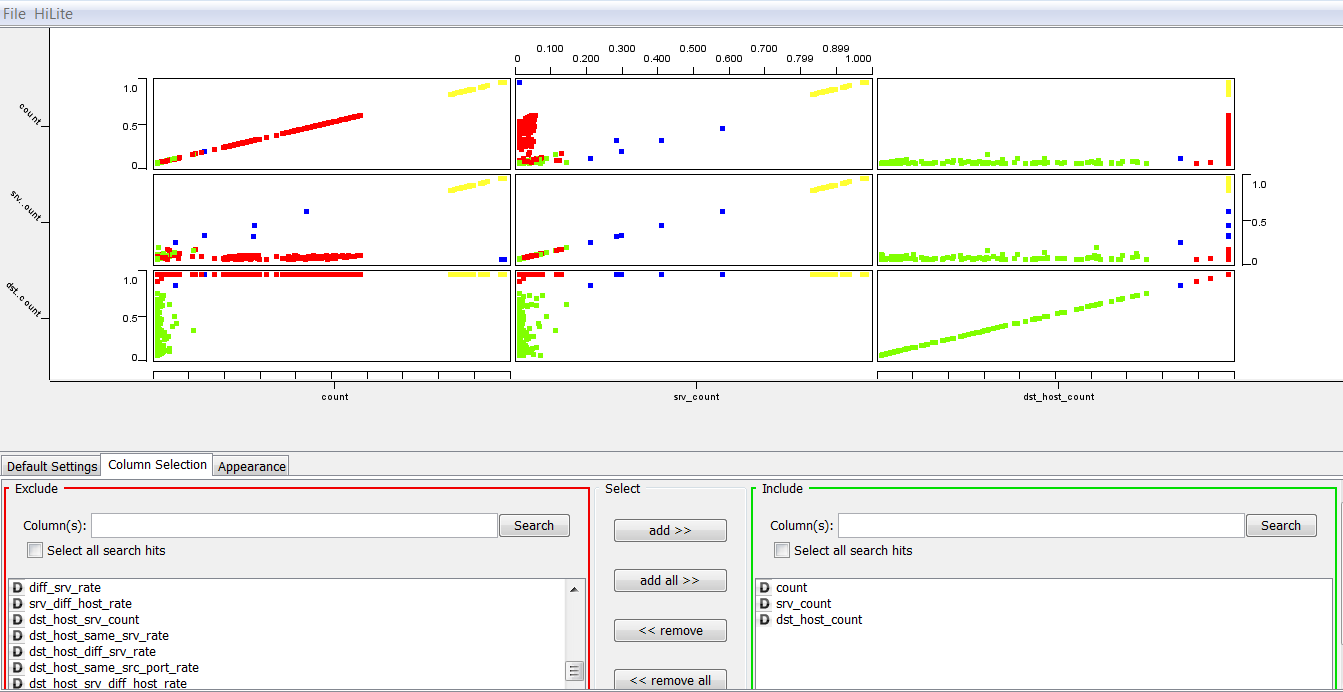
\includegraphics[width = \textwidth]{Klaster7}
slika 5.7: primer modela dobijenog primenom DBSCAN algoritma\\
\end{center}

Dobile smo druga\v ciji model u odnosu na prethodna dva puta, s obzirom na to da je DBSCAN algoritam zasnovan na gustini.\\
Sva tri algoritma su nam dala dobre modela, koliko je mogu\' ce uzev\v si u obzir prirodu na\v sih podataka.

\section{Klasifikacija}

Pre klasifikacije prvo smo u\v citali podatke, potom smo izdvojili 10\% skupa zbog brzine, a potom smo podelili podatke na trening i test skup, gde smo podesili da trening iznosi 70\% ukupnog skupa, a test 30\%. Bilo je neophodno izvr\v siti normalizaciju zbog knn algoritma i nakon toga smo mogli da primenimo algoritme za klasifikaciju. Koristile smo \v cetiri algoritma, kojima smo izdvojile preciznost i spojile ih u jednu tabelu da bismo lak\v se mogle da vidimo koji algoritam je najbolje klasifikovao na\v se podatke.

\begin{center}
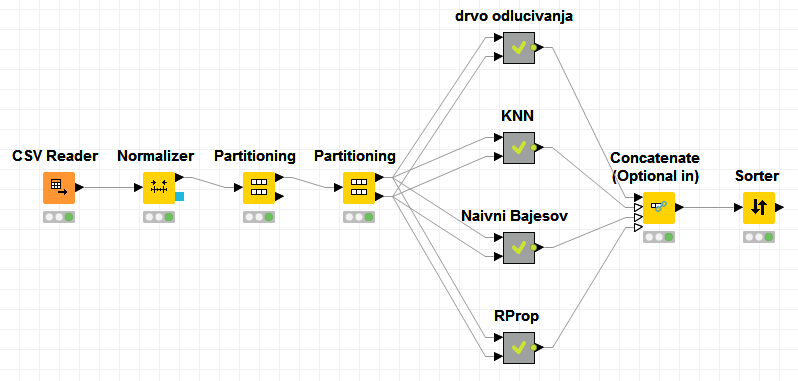
\includegraphics[width = \textwidth,height = 3.5 cm]{Klas1}
slika 6.1: klasifikacija\\
\end{center}

Prvi algoritam za klasifikaciju koji primenjujemo je drvo odlucivanja. Ne znamo na koliko treba da postavimo vrednost parametra Min number records per node tako da prvo u petlji (\v cvor Interval Loop Start) postavljamo da nam se vrednost promenljive menja u svakoj iteraciji od 1 do 10. 

\begin{center}
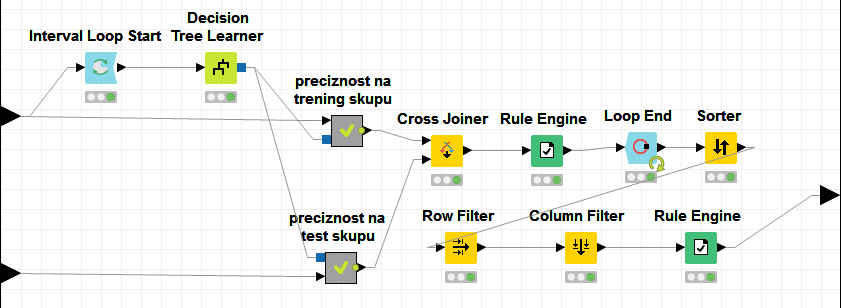
\includegraphics[ scale = 0.8]{Klas2_DO1}
slika 6.2: drvo odlu\v civanja\\
\end{center}

Nakon toga pokre\' cemo \v cvor Decision Tree Learner kome smo prethodno parametre podesile na slede\' ci na\v cin:

\begin{center}
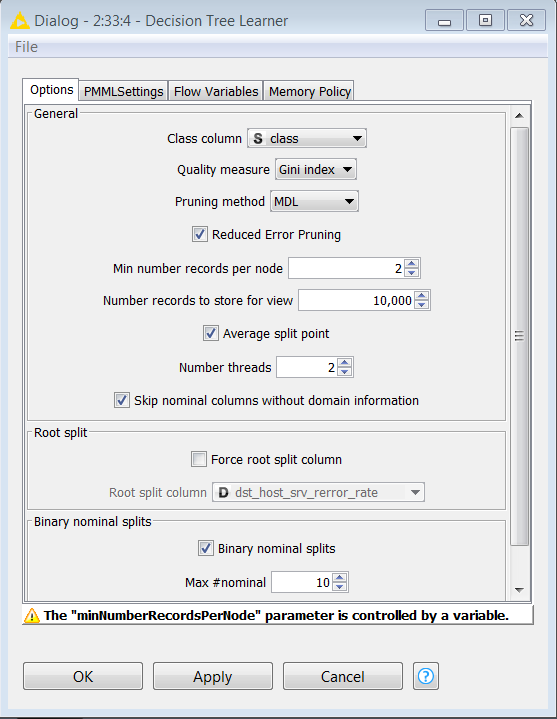
\includegraphics[scale = 0.75]{Klas3_DO2}\\
slika 6.3: pode\v savanje parametara \v cvora Decision Tree Learner\\
\end{center}

Kao rezultat dobijamo slede\' ce drvo odlu\v civanja:

\begin{center}
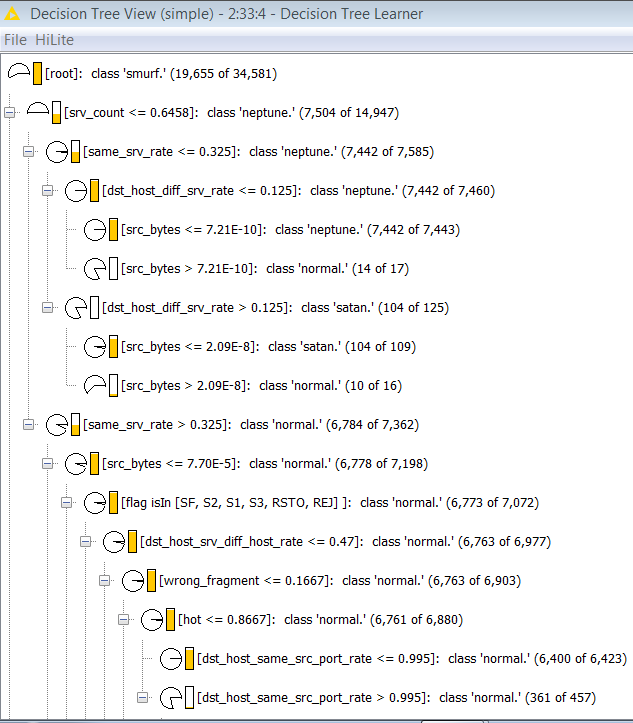
\includegraphics[width = 6 cm, height = 9cm]{DO1}
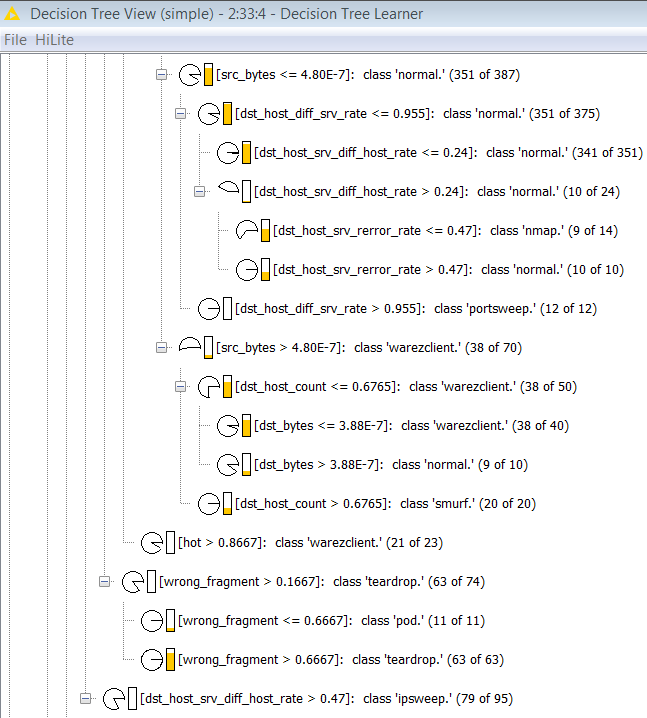
\includegraphics[width = 6 cm, height = 9cm]{DO2}
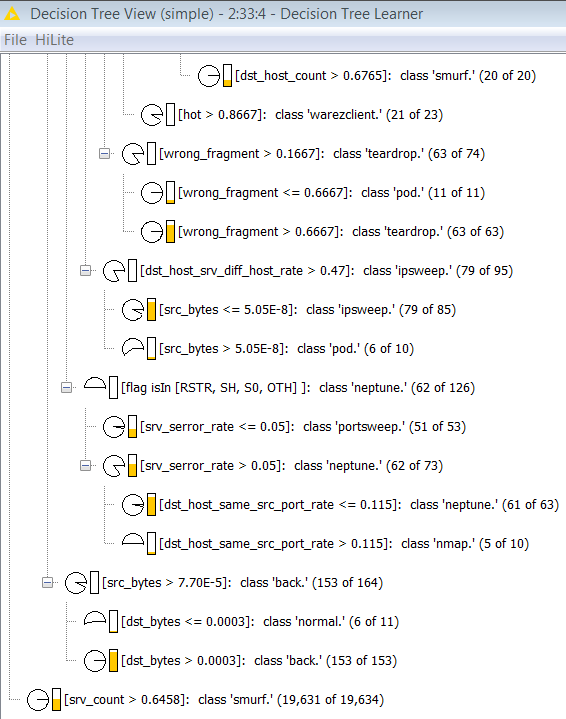
\includegraphics[width = 6 cm, height = 9cm]{DO3}\\
slika 6.4: izlaz iz \v cvora Decision Tree Learner - drvo odlu\v civanja\\
\end{center}

Slede\' ce \v sto \v zelimo je da dobijeni model primenimo na trening i test podatke i izdvojimo preciznost modela. U oba slu\v caja (slika 6.5 i slika 6.6) smo primenili sli\v can metod. Uz pomo\' c \v cvora Decision Tree Predictor smo dobijeni model primenuli na trening (test) podatke, a potom smo Scorer-om izdvojili matricu konfuzije i va\v zne statistike modela. S ozbzirom na to da se u koloni Accuracy nalazi samo jedan red sa vredno\v s\' cu preciznosti na\v seg modela, a ostala polja su nedostaju\' ce vrednosti, \v cvorom Row Filter smo izdvojili samo taj relevantan red. Column Filter-om smo izdvojili samo kolonu Accuracy a potom je Column Rename-om preimenovali u AccuracyTrening da bismo kasnije razlikovali preciznost trening od test skupa. Jedina razlika izmedju ova dva skupa je to \v sto za test skup nismo koristili Column Rename jer nije bilo potrebe, ako smo jednu preciznost nazvali AccuracyTrening drugu \' cemo znati da je preciznost test skupa.

\begin{center}
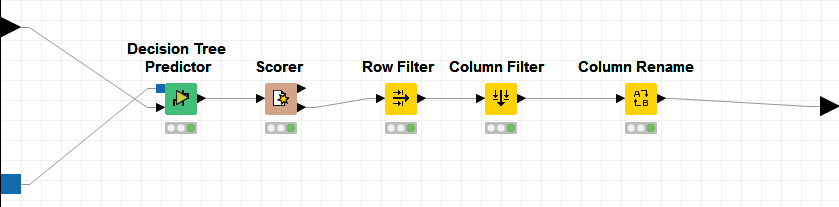
\includegraphics[width = \textwidth]{PnaTrening}
slika 6.5: preciznost na trening skupu\\
\end{center}

\begin{center}
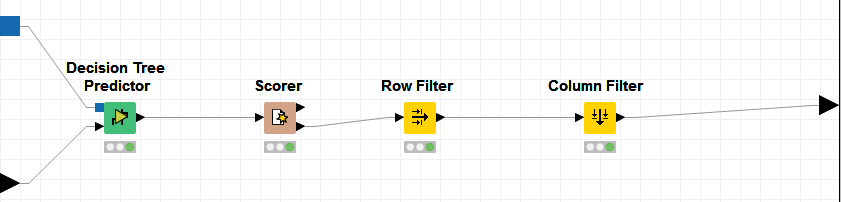
\includegraphics[width = \textwidth]{PnaTest}
slika 6.6: preciznost na test skupu\\
\end{center}

Nakon izra\v cunatih preciznosti oba skupa spajamo ih u jednu tabelu Cross Joiner-om, a Rule Engine-om dodajemo kolonu u tabelu koja sadr\v zi vrednost promenljive Min number records per node. \v Cvor Loop End prikuplja podatke iz svih iteracija petlje i dobijamo preciznost trening i test skupa za sve vrednosti promenljive, a potom \v cvor Sorter sortira redove opadaju\' ce po preciznosti test i trening skupa, respektivno. Rezultate mo\v zemo videti na slici 6.7.

\begin{center}
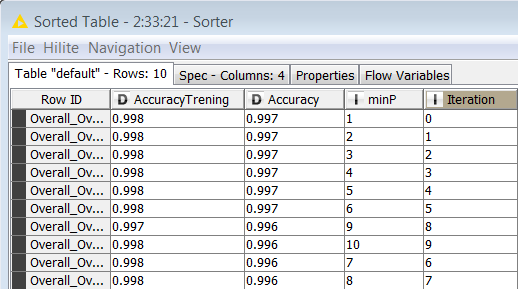
\includegraphics[scale = 0.5]{PoslePnaTest}\\
slika 6.7: preciznost test i trening skupa u odnosu na vrednost promenljive\\
\end{center}

Vidimo da je preciznost najve\' ca za vrednosti 1-6 promenljive Min number records per node.\\
Potom Row Filter-om izdvajamo prvi red - red sa najboljom precizno\v s\' cu, Column Filter-om izdvajamo kolonu Accuracy, a Rule Engin-om dodajemo kolonu koja ozna\v cava model koji smo koristili. Dakle, preciznosti smo dodali model za koji smo je dobili. Izlaz iz ovog \v cvora predstavlja ulaz u \v cvor Concatenate (Optional in) u koji \' cemo ubacivati i preciznosti ostalih modela kako ih budemo dobijali.\\~\\
Slede\' ci algoritam koji primenjujemo je k najbli\v zih suseda (KNN). Procedura je veoma sli\v cna kao i kod drveta odlu\v civanja sa razlikom \v sto smo ovde kroz petlju menjale vrednost k, i to od 3 do 15 sa korakom 2 (da bi vrednost uvek bila neparna). Takodje, K Nearest Neighbors radi samo na test skupu tako da smo ovde na kraju izdvojile samo preciznost test skupa, koja nam je, u su\v stini, jedina i bitna.

\begin{center}
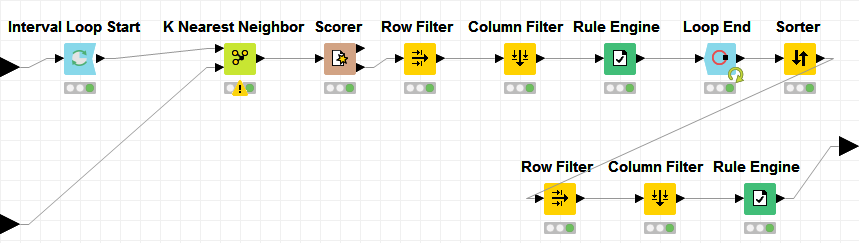
\includegraphics[width = \textwidth,height = 4.5 cm]{KNN1}
slika 6.8: KNN\\
\end{center}

Loop End je ponovo prikupio rezultate svih iteracija petlje i Scorer-om smo sortirali tako da na vrhu bude najbolja preciznost.

\begin{center}
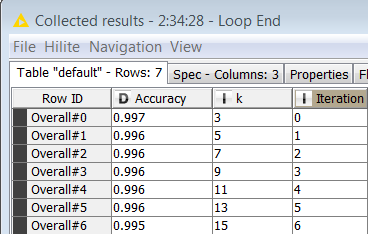
\includegraphics[scale = 0.8]{KNN2}\\
slika 6.9: preciznost test skupa u odnosu na vrednost parametra k\\
\end{center}

Naredni algoritam je Naivni Bajesov. Procedura je skoro ista kao i kod drveta odlu\v civanja, sem \v sto nemamo petlju u kojoj menjamo vrednost parametra.

\begin{center}
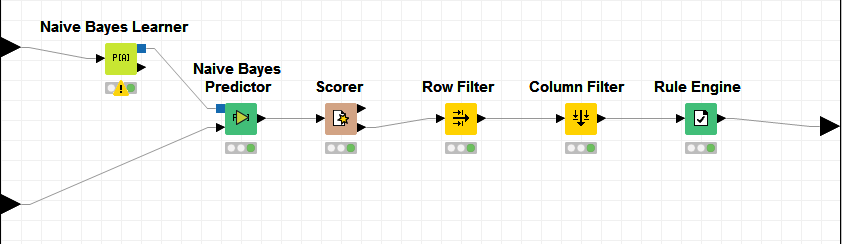
\includegraphics[width = \textwidth]{NB1}
slika 6.10: Naivni Bajesov\\
\end{center}

Parametre \v cvora Naive Bayes Learner postavljamo na slede\' ci na\v cin:

\begin{center}
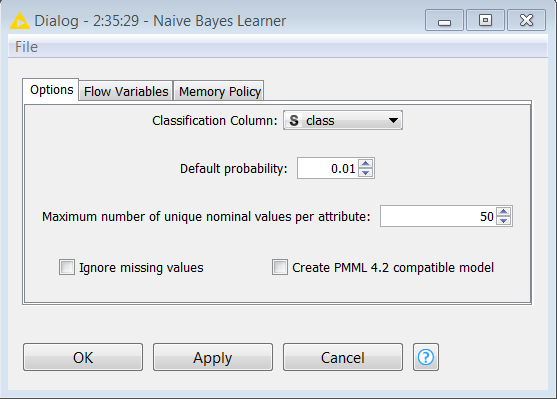
\includegraphics[scale = 0.5]{NB2}\\
slika 6.11: pode\v savanje parametara \v cvora Naive Bayes Learner\\
\end{center}

Poslednji algoritam klasifikacije koji smo koristile je algoritam neuronskih mre\v za RProp MLP. S obzirom na to da on radi isklju\v civo sa numeri\v ckim podacima prvo je bilo potrebno izbaciti kategori\v cke atribute, \v sto smo postigli \v cvorom Column Filter.

\begin{center}
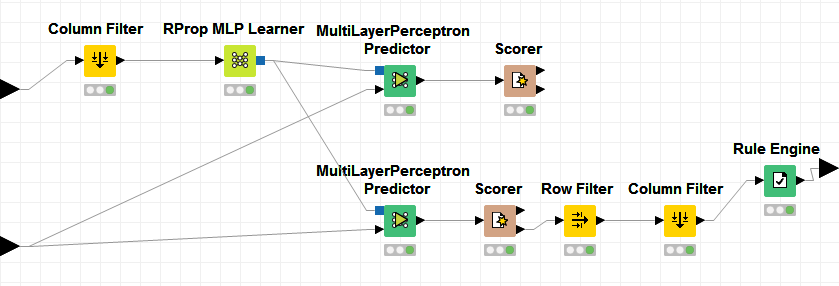
\includegraphics[width = \textwidth,height = 6 cm]{RPROP1}
slika 6.12: RProp\\
\end{center}

Parametre \v cvora Naive Bayes Learner smo postavili na slede\' ci na\v cin:

\begin{center}
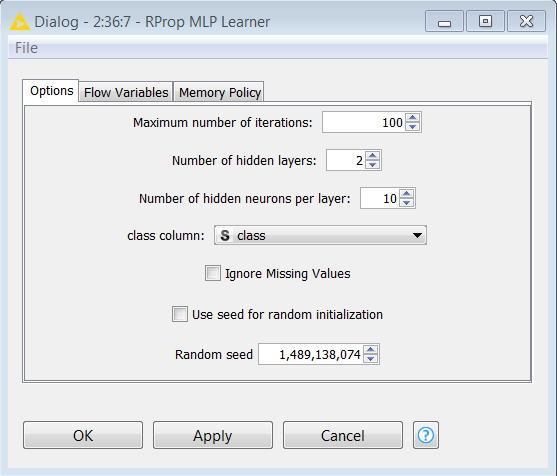
\includegraphics[scale = 0.5]{RPROP2}\\
slika 6.13: pode\v savanje parametara \v cvora RProp MLP Learner\\
\end{center}

U ovom slu\v caju smo model primenili i na trening i na test skup (kao i u slu\v caju drveta odlu\v civanja). Preciznost trening skupa je 0.997, ali nam ona nije bitna za dalji tako da smo je samo spomenuli ovde. \v Sto se preciznosti test skupa ti\v ce procedura je u potpunosti ista kao i u prethodnim algoritmima.\\~\\

Na kraju je jedino preostalo da spojimo dobijene preciznosti svih modela u jednu tabelu pomo\' cu \v cvora Concatenate (Optional in) i da ih Sorter-om sortiramo opadaju\' ce po preciznosti. Dobijeni su rezultati:

\begin{center}
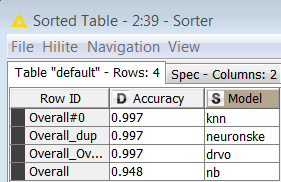
\includegraphics[scale = 0.75]{Finale}\\
slika 6.14: sortirane preciznosti dobijenih modela\\
\end{center}

Najbolju preciznost dobijamo u algoritmima KNN, RProp MLP, drvo odlu\v civanja, a neznatno manju u Naivnom Bajesovom. Ovako visok stepen nivo preciznosti nije iznenadjuju\' c s obzirom na to da imamo ciljnu klasu u tabeli i veliki broj numeri\v ckih atributa sa kojima mo\v ze da se barata. 

\end{document}
